\chapter{Relevante Grundlagen und Überblick über alternative Antriebe}
\label{ch:Relevante Grundlagen und Überblick über alternative Antriebe}
Für die Analyse der Forschungsfrage es ist wichtig die zentralen theoretischen Begriffe zu definieren. 
Das Kapitel \ref{s:Bodenabfertigungen eines Luftfahrzeugs} stellt die Grundlagen der Flugzeugabfertigung und 
die beteiligten Stakeholder am Flughafen dar. Zunächst beschäftigt sich das Kapitel \ref{s:Kosten}
mit den bedeutenden Informationen zu Kosten am Flughafen und Emission-Regulierungsinitiativen. 
Anschließend werden im Teil \ref{s:Neartige Antriebe}
die neuartigen alternativen Antriebe und dadurch betriebene Konzepte und Flugzeugmodelle vorgestellt.

\section{Stakeholder am Flughafen}
\label{s:Stakeholder am Flughafen}

Am Flughafen ist eine Vielzahl an Stakeholdern beschäftigt, die miteinander agieren. 
Durch die neuen Luftfahrzeugantriebe steht diesen Akteuren eine 
schwierige Aufgabe vor.\\

\textbf{Flughafen} \\
Einer der Stakeholder am Flughafen ist der Flughafenbetreiber selbst. 
Der Flughafen stellt der Fluggerät- und Passagierabfertigung Infrastruktur wie bspw. Terminals oder Start- und Landebahnen zur Verfügung (das gilt als Kernfunktion), 
wofür Nutzungsgebühren erhoben werden \cite{conrady2019luftverkehr}. %Seite 180, falls ich Entgelte durchzählen will.

Zum Flughafen gehören außer Start- und Landebahnen unter anderem Rollwege, Vorfeld, Flugsteige, sowie die Infrastruktur für die Gepäckabfertigung. 

Darüber hinaus stellen Flughäfen eine intermodale Verknüpfung dar \cite{conrady2019luftverkehr}. %d.h. die Anbindung an anderen Verkehrsmitteln wird hergestellt.
Direkte Nutzer von Flughäfen sind die Im- und Exporteure von Dienstleistungen und Waren \cite{schaar2010analysis}. 

Flughäfen sind ein großer Teil der regionalen Wirtschaft \cite{schaar2010analysis} und sorgen für eine Vielzahl an Arbeitsstellen. 
Dennoch verursachen sie ein Ausmaß an Lärm und Umweltbelastungen, die durch die Emissionen der Flugzeuge entstehen.
Demnach verlangt der Flughafen hierfür ebenfalls Entgelte. \\ %Kap 4

Für die Entwicklung der Infrastruktur und Begleichung der Betriebskosten müssen Flughäfen manchmal finanzielle Unterstützung aus anderen
Quellen, wie staatlicher Finanzierung, in Anspruch nehmen \cite{schaar2010analysis}.

Die Europäische Kommission besagt, dass Flughäfen mit einem Passagieraufkommen von über 3 Millionen 
Menschen p.a. in der Lage sind, ihre Betriebskosten selbst durch Gewinn zu decken. %Hier noch mal genauer werden

Eine Kategorisierung der Flughäfen basiert immer auf der Passagiermenge. Aufgrund dieser Kategorisierung für das Jahr 2023 gab es in Deutschland 
sieben große Gemeinschaftsflughäfen, einschließlich 2 Hubs, und 16 Regionalflughäfen (kleine und große).\footnote{Die Daten stammen aus dem Statistischem Bericht, Luftverkehr auf Hauptverkehrsflughäfen 2023} % keine ahnung ob dem oder einem
%Wobei die kleinere Flughäfen mehr Hilfe brauchen

Der Europäischen Kommission nach werden die Flughäfen nach jährlichem Passagieraufkommen folgend unterteilt: 
\begin{itemize}
    \item große Gemeinschaftsflughäfen > 10 Mio. Passagieren;
    \item nationale Flüge mit 5 bis 10 Mio. Passagieren;
    \item große Regionalflughäfen mit 1 bis 5 Mio. Passagieren;
    \item kleine Regionalflughäfen < 1 Mio. Passagieren.
\end{itemize}

„große Gemeinschaftsflughäfen“ mit über 10 Mio. Passagieren jährlich; 

\textbf{Fluggesellschaft} \\
Fluggesellschaften sind Dienstleister, welche die Infrastruktur eines Flughafens für die Abfertigung von Passagieren und Fracht nutzen. 
Sie sind gewinnorientiert und haben das Ziel wettbewerbsfähig zu bleiben. 
Für eine Fluggesellschaft ist von Relevanz, wie hoch die Betriebskosten (Erträge)
sind, die der Flughafen verlangt \cite{schaar2010analysis}. Die Erträge unterscheiden sich in Flughafengröße und Flugzeugtyp.

Fluggesellschaften und Treibstoff-Firmen sind für die sichere Betankung verantwortlich. Quelle: Annex 14 (Doc 9137 Teil 8)
\\
\textbf{Bodenverkehrsdienste} \\ %S. 183 conrady
Bodenverkehrsdienste sind für die Abfertigung der Flugzeuge auf dem Boden zuständig. 
Nach Conrady \cite{conrady2019luftverkehr} gehört zu ihren Tätigkeiten außerdem:  
die Fluggastabfertigung, administrative Abfertigung sowie Transportdienste.
Sie sind auf Infrastruktureinrichtungen wie Gepäckförderanlagen und Betankungsanlagen angewiesen. 
Die Abfertigung kann entweder von einer Fluggesellschaft, einem Flughafen oder einem unabhängigen Dienstleister durchgeführt werden. 
Meistens werden die Bodenverkehrsdienste in Deutschland von den Flughäfen übernommen. \\ %oder die externen Firmen (Dritte) werden engagiert.

Bodenverkehrsdienste sind auch für den Transport von Fracht, Post und Gepäck bis zum Flugzeug zuständig \cite{mensen2013handbuch}.

OPS 1.1150 "Handling agent. An agency which performs on behalf of the operator some or all of the latter's functions
including receiving, loading, unloading, transferring or other processing of passengers or cargo;"

%Von der Fluggesellschaft werden Handling Agents eingestellt, der die ganze Abfertigung und Kommunikation zwischen Beteiligten am Vorfeld
%kontrollieren.
%In dieser Arbeit werden nur die internationale und regionale Verkehrsflughäfen betrachtet. 
%(Es bietet sonstige Serviceleistungen für die Passagiere, wie Parkplätze, Handel Dienstleistungen.)

Zu den Systempartnern am Flughafen zählen ebenfalls Luftfahrzeughersteller, Flugsicherungen, Reiseveranstaltern, staatliche Institutionen \cite{maertens2023neue},
sowie Beteiligte wie Passagiere, Arbeitskräfte und Passagierdienstleister. 
Sie nehmen nicht direkt an der Flugzeugabfertigung bzw. an Betrieb am Vorfeld teil, deswegen werden sie nicht weiter betrachtet.
Analog hierzu wird die Flugsicherung aufgrund unveränderter Umstände durch alternative Antriebe nicht betrachtet. 
Die Arbeit wird sich auf die Betriebskosten einer Fluggesellschaft und Infrastrukturkosten des Flughafens fokussieren.


\textbf{Vorfelddienste}

Betankungsdienste führen nicht nur die Be- und Entladung und Lagerung durch, sondern auch für andere Flüssigkeiten (wie z.B. Öl) zuständig.
Wartungsdienste führen die routinemäßige Kontrolle den Flugzeugen vor den Flügen (line Maintenance).
Die Reinigungsdienste und der Flugzeugservice sind Reinigung von Innen und Außen eines Flugzeugs verantwortlich, Wasserservice, 
Klimaanlagen in der Kabine und Enteisung.


Auf die Kosten eingehen:
Laut OPS 1.175 %"The number of ground staff is dependent upon the nature and the scale of operations"
Anzahl der benötigten Bodenmitarbeiter ist von dem Maßstab der Operationen am Flughafen anhängig.


Gute Zusammenarbeit der Akteure/Stakeholder fördert die Pünktlichkeit der Abfertigung und hilft die 
Verspätungen zu vermeiden \cite{schmidt2016challenges}.

 
%BAs können weniger überlastete Flughäfen anfliegen und entferne Bereiche, und
%nur die geringe Bedarf abdecken.
%Europäische Kommission Leitlinien für staatliche Beihilfe für Flughäfen und Luftverkehrsgesellschaften 2014/C 99/03
%
%Als Regionalflughafen definiert E Kommissionen einen Flughafen mit bis zu 3 Millionen Passagieren im Jahr.
%Flughäfen mit mehr als eine Million Passagieren im Jahr decken überwiegend ihre Betriebskosten selbst. %egal?
%
„Betriebskosten“: die mit der Erbringung von Flughafendienstleistungen verbundenen Kosten eines Flughafens;
 dazu gehören Kostenkategorien wie Personalkosten, Kosten für fremdvergebene Dienstleistungen, Kommunikation, 
 Abfallentsorgung, Energie, Instandhaltung, Mieten und Verwaltung, jedoch weder Kapitalkosten, Marketingunterstützung 
 bzw. andere Anreize, die der Flughafen den Luftverkehrsgesellschaften bietet, noch Kosten für Aufgaben mit hoheitlichem Bezug;

 	
%Der Bedarf an öffentlichen Mitteln zur Betriebskostenfinanzierung variiert unter den derzeitigen Marktbedingungen
% aufgrund der hohen Fixkosten in der Regel je nach Flughafengröße und ist normalerweise bei kleineren Flughäfen
 % verhältnismäßig höher. Unter den derzeitigen Marktbedingungen können nach Auffassung der Kommission in Bezug auf
%   die jeweilige finanzielle Tragfähigkeit nachstehende Kategorien von Flughäfen abgegrenzt werden:

%d)Flughäfen mit 1 bis 3 Millionen Passagieren im Jahr dürften im Durchschnitt in der Lage sein, ihre Betriebskosten überwiegend selbst zu tragen;

%e)Flughäfen mit mehr als 3 Millionen Passagieren im Jahr erzielen in der Regel einen Betriebsgewinn und dürften 
%in der Lage sein, ihre Betriebskosten zu decken.


\section{Bodenabfertigungen eines Luftfahrzeugs}
\label{s:Bodenabfertigungen eines Luftfahrzeugs}

Zur Veranschaulichung der Änderungen an der Infrastruktur am Flughafen die durch neuartige Antriebe vorgenommen werden müssen, 
ist es notwendig wichtige Begriffe einer Abfertigung des konventionellen Flugzeugs hervorzuheben (definieren). 
Unter konventionellen Luftfahrzeugen sind die zu verstehen,
die mit fossilen Treibstoffen, wie Kerosin, betrieben werden. Der Fokus wird auf die gewerblichen Passagier-Flugzeuge gelegt,
weil die Abfertigung von Passagieren besonders strengere Sicherheitsmaßnahmen erfordert.

%Nach der Reinigung der Kabine (Boeing B747-400 im Transit bis zu 45 min), Toiletten und Frischwasser nachfüllen und Catering
%Boarding ca. 15-20 min pro 100 PAX

Die Blockzeit setzt sich aus der Zeit vom Beginn der Bewegung von der Parkposition bis zum Ende der Bewegung zur Parkposition, 
einschließlich der Flugzeit, zusammen.

An der Parkposition des Flughafens werden die Triebwerke ausgeschaltet und der Ablauf eines Turnaround beginnt. 
Mensen \cite{mensen2013handbuch} definiert den Turnaround, wie die Abfertigung der Flüge, die zeitnah zusammen liegen.
Bei einem Turnaround wird das Luftfahrzeug durch viele Akteure am Flughafen, wie Flugplatzbetreiber, Fluggesellschaft und die Dritte, für 
den nächsten Flug vorbereitet \cite{mensen2013handbuch}. Es muss ausgeladen, kontrolliert, gereinigt, anschließend versorgt 
und für den nächsten Flug beladen werden. \\
\\
Die Abbildung \ref{abfertigung} stellt die Abfertigung eines Flugzeugs an der Parkposition dar.
Nach ICAO Doc 9157: besteht Abfertigung eines Passagierflugzeugs aus Passagier-, Gepäck- und Frachtabfertigung, 
Sanitärservice, Wasserbetankung, Gepäckabfertigung, Betankung, Stromversorgung,
Startluft?, Schleppen von Flugzeugen, Bordküchenservice, Wartungsservice sowie Bereitstellung einer Klimaanlage und Sauerstoff,
wie in der Abbildung dargestellt.

Das Flugzeug wird an ein Hilfstriebwerk (auxiliary power unit - APU) angeschlossen \cite{mensen2013handbuch}. 
Die APU liefert Strom, wenn die Haupttriebwerke nicht laufen (quelle: [Annex 14. Doc 9137 Part 8]).
Parallel werden Fracht und sonstige Gepäckeinheiten mit dem Hubwagen abgeladen und mit Transporthängern zur Sortieranlage 
im Terminal gebracht \cite{mensen2013handbuch}. Im Falle, das die Parkposition direkt am Flughafen ist, 
können Passagiere direkt über die Treppe oder Fluggastbrücke zum Terminalgebäude gelangen. 
Wenn die Parkposition am Vorfeld liegt, muss auf einen Bus zurückgegriffen werden. 
Laut EU-OPS 1.305 darf das Luftfahrzeug aus Sicherheitsgründen erst betankt werden, wenn die Passagiere sich nicht an Bord befinden. 
%ICAO empfiehlt in Annex 6, dass Flugzeuge sollen erst betankt werden, wenn alle Passagiere raus sind 
%Das Flugzeug wird abgefertigt und wenn die Flüge zeitnan zusammen liegen beginnt ein Turn Around (TA) \cite{mensen2013handbuch}, 

\begin{figure}[h]
	\centering
	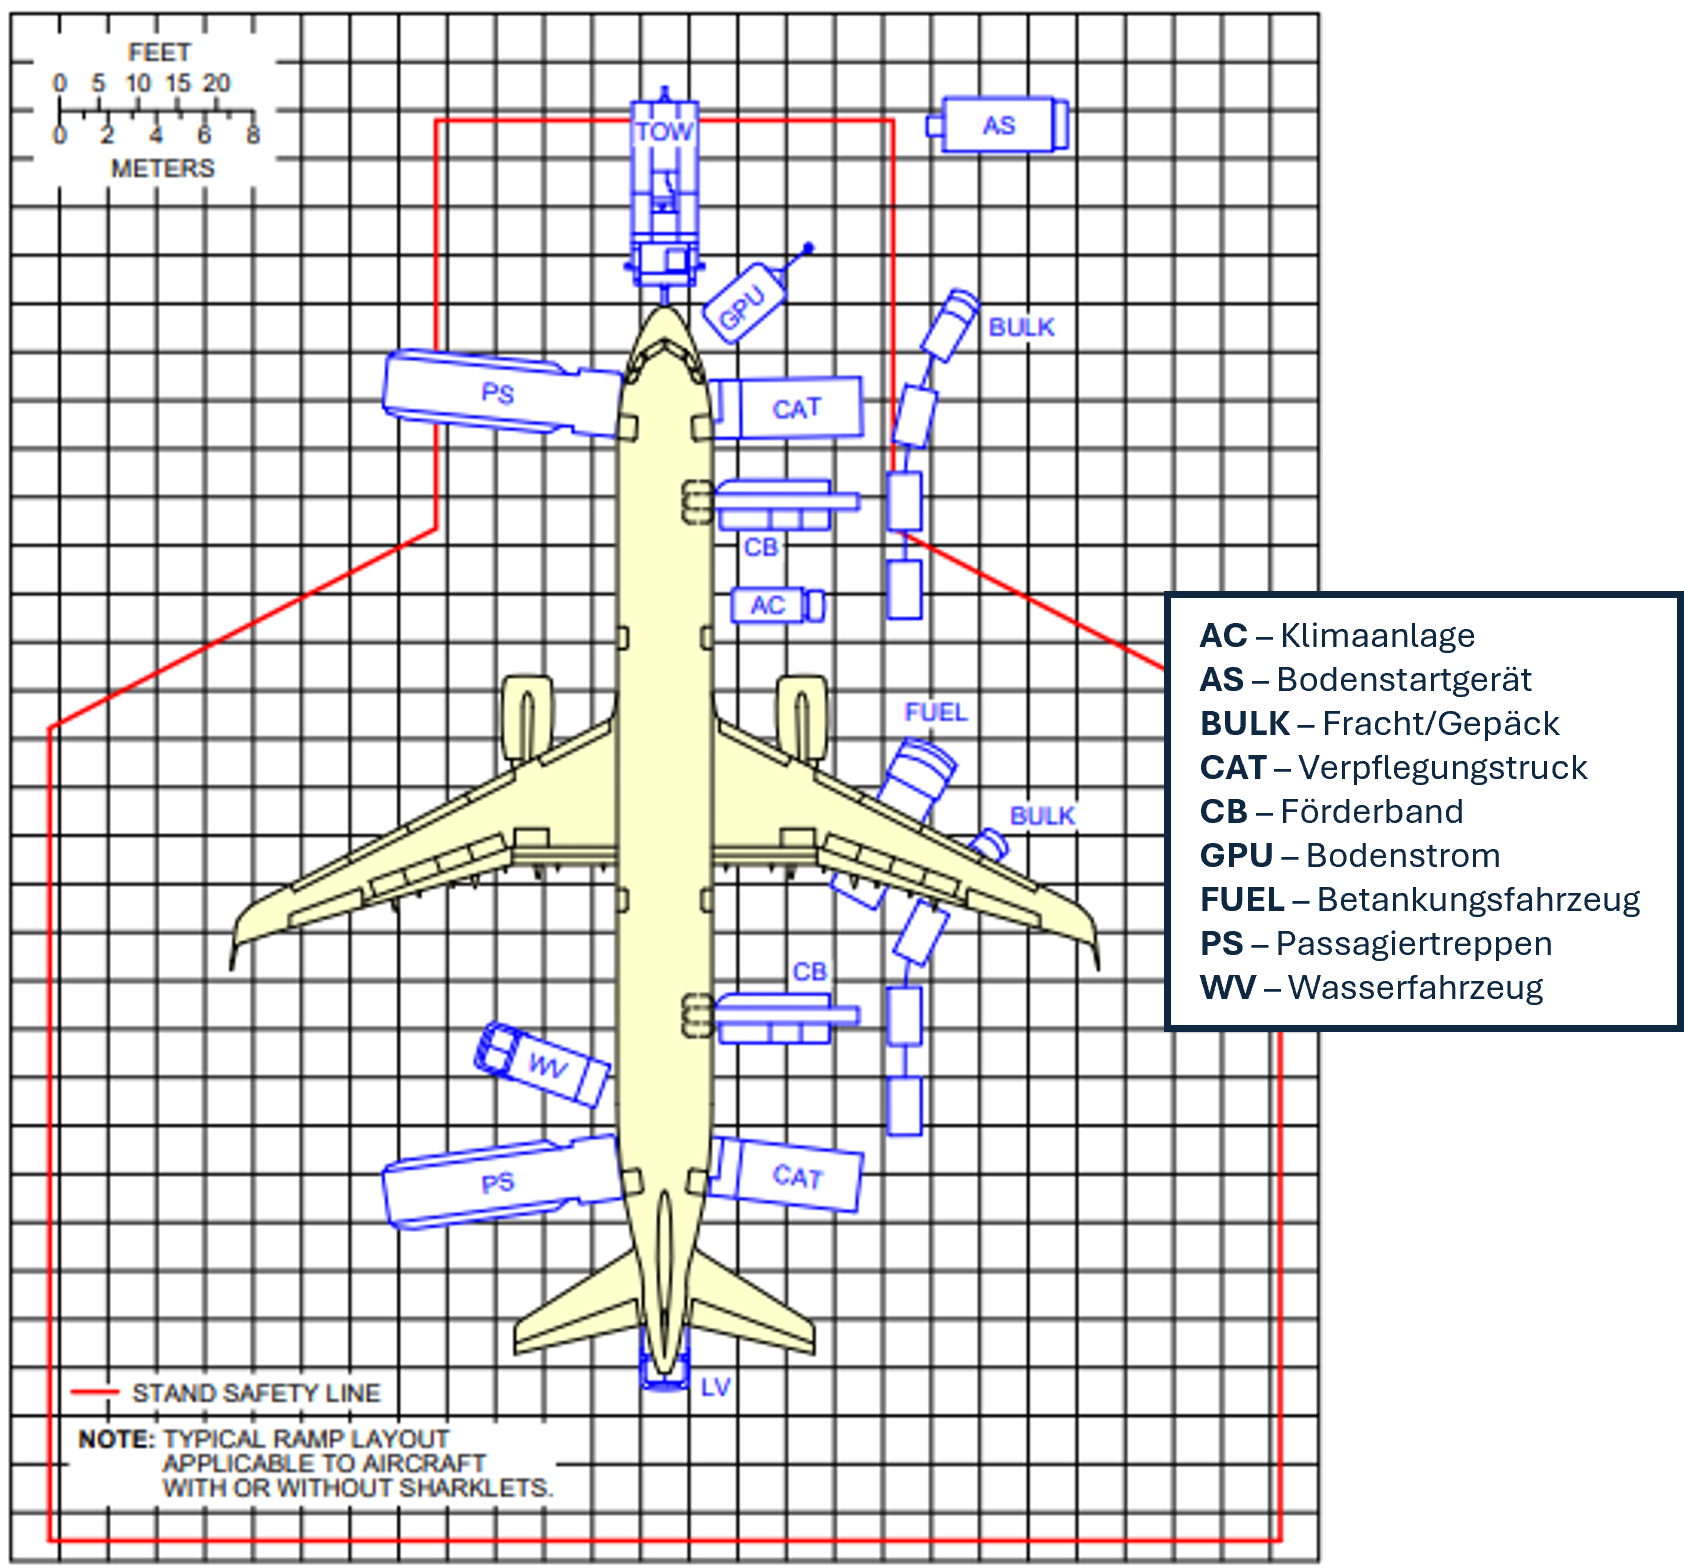
\includegraphics[width=0.8\linewidth]{Bilder/A321_Abfertigung.png}
	\caption[Abfertigung]{Abfertigung eines A321 \cite{airbus2022a321} mit eigenem Hinweis}
	\label{abfertigung}
\end{figure}

%"Die TurnaroundTime ist die Zeit vom Andocken des Flugzeugs amGate bis zumAbrollenvomGate." \cite{conrady2019luftverkehr} S 368

%Fluggast- Fracht-, und Postabfertigung 
%Fluggastabfertigung beinhaltet alles um den Service für die Passagiere.

Je nach Flugdistanz und nach Flugzeuggröße kann es zu unterschiedlichen Abfertigungszeiten kommen. Bei einem kleineren Flugzeug ist die Dauer 
kürzer als bei einer größeren Maschine. 
In Bezug auf die Transportdistanz unterscheidet man nach Kurz- (ca.2 Stunden oder bis 1000 km) 
und Mittelstreckenflüge (bis 3,5 Stunden oder bis 3000 km), Langstreckenflüge (ab 3,5 Stunden und ab 3000 km) \cite{mensen2013handbuch}.
Der Flughafen Frankfurt definiert jedoch die Transportdistanz anders, diese Werte werden auch im Kapitel \ref{s:Betriebsszenarien} genutzt.



